


\chapter{Abstraction Blocks: Thinking with Boxes for Flexible Abstraction \& Collaboration}
% \chapter{Thinking with Boxes: Tools for Abstraction Enable Flexible Creative Work}
\label{chapter:abstraction}
\begin{quote}
Effectively communicating ideas is an important part of creative collaboration, particularly in getting started and generating ideas. One major challenge of collaboration is the pull of concrete details over conceptual concerns as concrete details often stand out more than high-level structure. For example, discussing specific details of a drawing early can pull attention away from assessing whether the drawing's composition works as a whole. This chapter investigates using a strategy called \textit{abstraction blocks}, movable shapes to represent size and position of drawing elements without the need (or ability) to specify concrete details, for collaborative drawing. We hypothesized that structuring abstraction around these blocks enables more flexible exploration and communication. In an observational study of six synchronous small groups ($n=19$) sketching collaboratively, we found that abstraction blocks enabled more iterative and flexible exploration of drawing compositions. Groups using abstraction blocks explored alternative drawing compositions and discussed high-level concepts such as point-of-view and scale compared to sketching alone.
\end{quote}

\section{Introduction}
% Making Abstraction Concrete
We communicate with others at all stages of creative work, from ideation to critique \cite{mamykina2002collaborative}. 
For example, when writing, collaborators often first generate a high-level outline, later shifting focus to a lower level by revising grammar \cite{sommers1980revision}. Visual work like web design also spans abstraction levels, from task goals to deciding specific element placement \cite{klemmer2001designers}. Early on, high-level concerns should dominate. For example, in drawing, exploring various compositions early is more important than deciding what specific characters look like. Lightweight sketches serve as exploratory tools to visually communicate ideas in domains from architecture to illustration \cite{Buxton2007,Tversky2011,Tversky2009}. Dancers use marking to physically think through choreography without focusing on the details of the dance \cite{kirsh2011marking}. Designers use paper prototyping \cite{Snyder2003} and storyboarding \cite{landay1996sketching} to collaboratively think through a goal without focusing heavily on concrete details. These `blocking' strategies help people view work as high-level chunks rather than individual elements \cite{Chase1973,Gobet1998,chi1981categorization} While abstract chunking and high-level exploration are important for both ideation and collaboration, the emphasis of online collaboration in creative tasks has been on refinement and revision of completed work. Focusing on details early on can shift a group's attention to refinement rather than rough exploration, which can lead to fixation on a single idea \cite{jansson1991design,simon1972theories} or iterating incrementally on a previous idea rather than trying a potentially new and better concept \cite{Dow2009,Little2010,Yu2016}. 

We know that abstraction helps \emph{individuals} focus on high-level concerns \cite{Chase1973}; a combination of early stage abstraction and structure may also help \emph{collaborators} focus on high-level ideation and communicate with one another. We hypothesize that explicitly supporting `chunks' for early-stage design catalyzes collaborators' ability to revise at an appropriate level of abstraction by breaking down sketches into discrete, adaptable parts. Inspired by expert uses of chunking and tools that use tangible interfaces and techniques \cite{klemmer2001designers,Resnick2009}, this chapter investigates using abstract blocks as a form of visual chunking and a tool for structuring group communication. 
For example, a drawing of a tourist at a train station might consist of several abstract blocks to represent placement of these elements (Figure \ref{fig:blocks}); these blocks can be directly manipulated to communicate desired changes, suggestions, or ideas without the immediate need to change the sketch itself. Users can choose to label the blocks either through text or pictorially, giving flexibility in how they choose to represent their ideas. We focus on sketching as an initial exemplar domain of the broader class of creative work because sketching is an easily accessible medium that only requires pen and paper and is a beneficial tool for visual communication \cite{Buxton2007,Tversky1999}.

\begin{figure}
\centering
  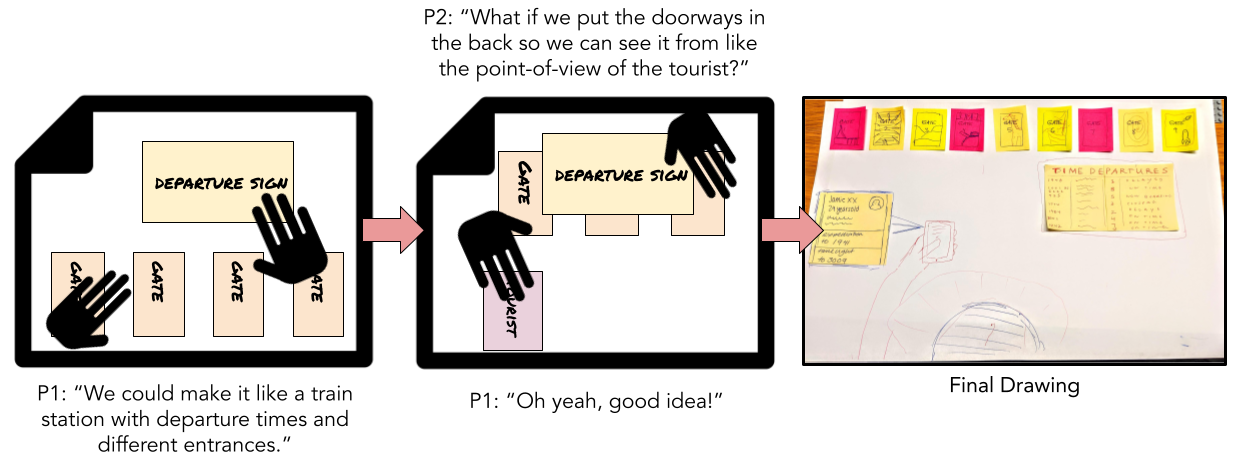
\includegraphics[width=\textwidth]{abstraction/figures/main_fig.png}
  \caption[A group from our study discussed composition and layout ideas for a collaborative sketch using abstract blocks.]{A group from our study discussed composition and layout ideas for a collaborative sketch using abstract blocks. These tangible and malleable blocks remove the need for smaller details and emphasize exploration. The prompt for the sketch was ``A scene with a time-travelling tourist.''}~\label{fig:blocks}
\end{figure}

% We hypothesize that this form of structured abstraction helps groups break down sketches into discrete, adaptable parts to communicate high-level ideas.
%---
%THINKING WiTH BOXES

An observational study investigated abstract blocks in a collaborative task. Six groups of novices ($n=19$) created drawings collaboratively. We audio and video recorded sessions and interviewed groups in a retrospective think-aloud. Groups used a paper implementation of abstraction blocks, using sticky notes, to plan a sketch based on a prompt. Working with simple blocks helped groups to see their drawings in terms of malleable, conceptual chunks. Tangible blocks helped groups discuss high-level concepts like `point-of-view` or `scale` and helped them quickly explore and change the composition of the drawing by editing the configuration of the blocks. Working at this more abstract, block level appeared to keep early discussion on more conceptual discussion rather than lower-level implementation details. These results suggest to us that offering (or even enforcing) abstract creation primitives like blocks catalyzes an emphasis on strategic and conceptual issues. 


\section{How is Abstraction Used in Creative Work?}

One definition of abstraction is that higher-level features are stable and static whereas lower-level features are those that can change in context \cite{shapira2012levels}. From an information storage perspective, high-level abstractions form units of information, or chunks, formed from recognized patterns \cite{Chase1973,Gobet2001,Gobet1998}. Early in creative work, higher-level abstractions enable the exploration of concepts rather than details such as when dancers use marking to think through an overall choreography \cite{kirsh2011marking} or when illustrators or designers use preliminary sketches to communicate rough thoughts \cite{Buxton2007, landay1996sketching, Tversky2011,Tversky2009}. Rubrics and templates are other forms of abstraction tools because they highlight structural goals that are adapted and refined through the addition of concrete details \cite{andrade2005teaching,yuan2016}. While experts utilize abstraction techniques like sketching to explore and engage in a reflective dialogue with others and their work \cite{schon1984reflective,Tversky1999,Tversky2009}, novices are often drawn to details \cite{jansson1991design,marsh1996examples,Smith1993}. Particularly in visual creative work, this may be because novices are hesitant of their drawing ability or perceive even sketching to be more permanent \cite{Hennessey,welch2000sketching}. This chapter presents abstraction blocks as a strategy for malleable, high-level chunking in visual creative work that eliminates the necessity for early-stage sketching. 

\subsection{Limited Support for Abstraction in Collaborative Creative Tools}
%TOOLS FOCUS ON DETAILS INSTEAD OF ABSTRACTION
Particularly for online collaboration in creative work, tools and strategies for abstraction are limited. Many online projects take a crowdsourcing workflow approach, breaking down larger projects into smaller microtasks with a global goal to ensure coherence even in asychronous collaborations \cite{Hahn2016}. For text-based projects such as writing a collaborative story, workflows that decompose the work into concrete chunks and allow for interdependent contributions can facilitate structured, high-quality work \cite{Kim2016,Kim2017,Retelny2014,Salehi2018,Valentine2017}. Visual creative work like drawing is similar to that of written work in that an overall theme and composition need to be developed to create a cohesive final artifact, but while text has inherent sequential structure, images are not linear and not as easily broken down into independent workable parts \cite{Johnson-Laird1983}. 

Communication of abstract ideas within these collaborations may rely more on coordinating actions and developing rapport \cite{Davis2017,Davis2016}, which can be difficult in online settings where groups must rely on technological affordances to effectively communicate \cite{Hollan1992,Jensen2018}. Strategies for abstraction in collaborative visual work are limited in implementation. For example, SwarmSketch \cite{swarm} allows users to influence the direction of a collaborative drawing by contributing a single ink stroke however they like, but does not provide tools for communication between contributors or structure for how work should be coordinated. As a result, many drawings become a haphazard collection of strokes that no longer match the original goal and are difficult to change \cite{Boxer2005}. The Johnny Cash Project \cite{TheJohnnyCashProject2012} also predefines the overall project goal of collaboratively making a hand-drawn music video and coordinates contributor work through individual tasks (such as tracing over a designated image); however, it necessarily limits contributions to a single level of detail for ease of coordination, preventing contributors from influencing the direction of the project as a whole. 

\begin{figure}
\centering
  %\vspace{-0.2in}
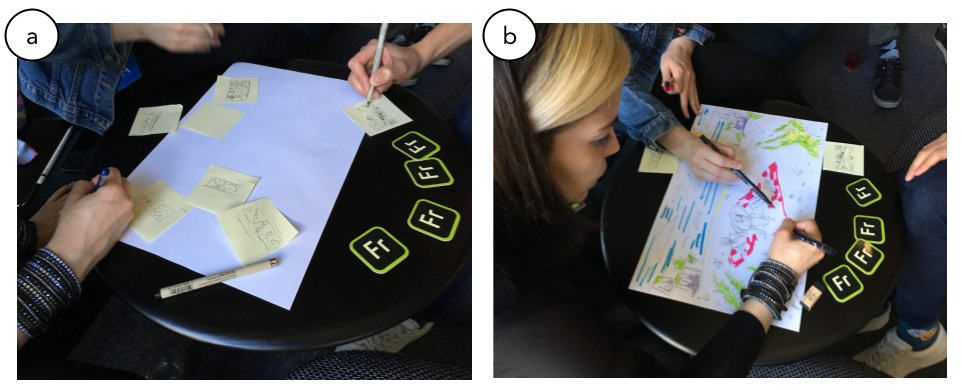
\includegraphics[width=\textwidth]{abstraction/figures/expert.png}
\vspace{-0.2in}
  \caption{a) Experts started planning by sketching multiple thumbnails that conveyed overall structure and composition more than details. b) These composition sketches provided a reference for experts during drawing.}
  ~\label{fig:expert}
  \vspace{-0.2in}
\end{figure}

``Blank page'' tools allow for open-ended abstraction, but are often unstructured. The problem with remaining too abstract or unstructured, especially in collaborative work, is that communication and consensus may get lost in the woods \cite{hinds1999curse,hinds2001}. Multiplayer experiences such as those in  Figma (www.figma.com), Google Docs \cite{wang2015students}, or collaborative drawing canvases (www.drawpile.net) enable a large range collaboration strategies, from allowing anyone to modify anything through pixel-perfect editing, to splitting the canvas or document into sections and assigning collaborators to each part. Digital whiteboards \cite{Ishii1992} and sketch interfaces \cite{lin2000denim} similarly give users the freedom to express their thoughts with as much or as little detail as desired. However, these systems leave it to the users to develop their own external collaboration structures. Without prerequisite knowledge of abstraction strategies, novices especially may continue to lean towards specific details, such as the exact specifications of a sketch \cite{welch2000sketching} or precise wording of an essay \cite{sommers1980revision}. Abstraction blocks ground the exploration and communication of abstract ideas to movable boxes to shift focus away from low-level details while giving tangible artifacts with which to interface.

\section{Abstraction Blocks: Thinking with Boxes}

\subsection{Formative Interviews: How Do Experts Collaborate?}
To investigate the role of abstraction in how experts communicate during collaboration, we observed three proficient illustrators recruited from a local drawing and illustration club perform a collaborative drawing task. In this task, the group made a single drawing together based on an open-ended prompt, ``Draw a scene of a place that makes you happy.'' We provided the group with paper, sticky notes, pencils, colored pens and markers, and a single large sheet of paper as the canvas for their drawing. We observed that experts used abstraction in three main ways.

First, experts used abstraction to quickly capture ideas from members of the group. In planning their drawing, the group first created several small thumbnail sketches on sticky notes as members generated ideas for various drawing compositions as part of their planning process (Figure \ref{fig:expert}). Creating small, abstract drawings is a common technique for visually generating ideas and solving problems \cite{poore1967composition,Poore1967}. In this collaborative context, this technique additionally functioned as a way to communicate and confirm thoughts between members of the group, throwing out various ``what if'' scenarios: \textit{``What if we made like ice cream dogs? I know that's silly, but it conveys happy.''} Sometimes a participant would sketch a thumbnail themselves and place it in the center to show the group their idea. Other times, a participant would draw a thumbnail sketch as a different participant was verbally describing their idea, while asking for confirmation that their sketch of the idea was accurate. In a post-interview, the experts mentioned that they learned the thumbnailing technique from their art education and practice.

\begin{figure}
\centering
  %\vspace{-0.2in}
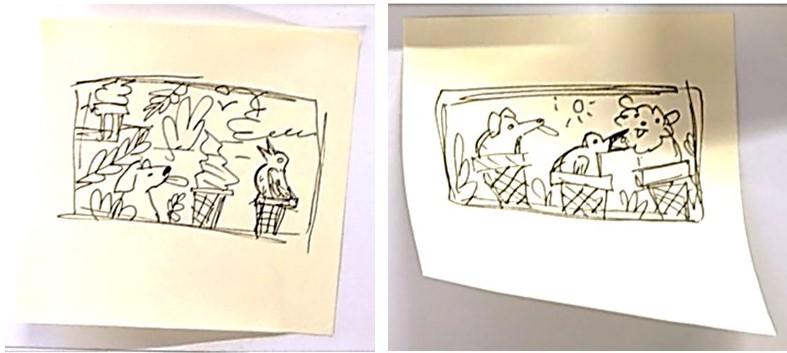
\includegraphics[width=\textwidth]{abstraction/figures/thumbnails.jpg}
\vspace{-0.2in}
  \caption{An expert participant sketched these two thumbnails to illustrate and explore alternate compositions for similar elements.}
  ~\label{fig:thumbnail}
  \vspace{-0.2in}
\end{figure}

Second, experts used abstraction to reduce unnecessary work by reusing elements that had already been drawn. For example, Figure \ref{fig:thumbnail} shows two thumbnail sketches that contain similar elements in different layouts and compositions. To choose a direction for their sketch, the group placed the thumbnail sketches in front of them and discussed to come to a consensus. These sketches conveyed relative positioning of sketch elements rather than specific details of the drawing. The group decided on an overall composition while adding in ideas contributed through other group members' thumbnails.

Lastly, experts used abstraction as a way to anchor discussions about how to proceed.
After deciding on an overall composition, the expert group  assigned work to each of its members. However, rather than assigning work based on areas of the canvas paper, the group delegated work based on the elements in the composition they had developed together: ``\textit{You draw the background since it's your design, you draw the foliage, and I'll draw the [character]?}'' This gave a clear sense in who would draw which part of the sketch and drew from their rough composition plan. 

% \begin{figure}
% \centering
%   %\vspace{-0.2in}
% 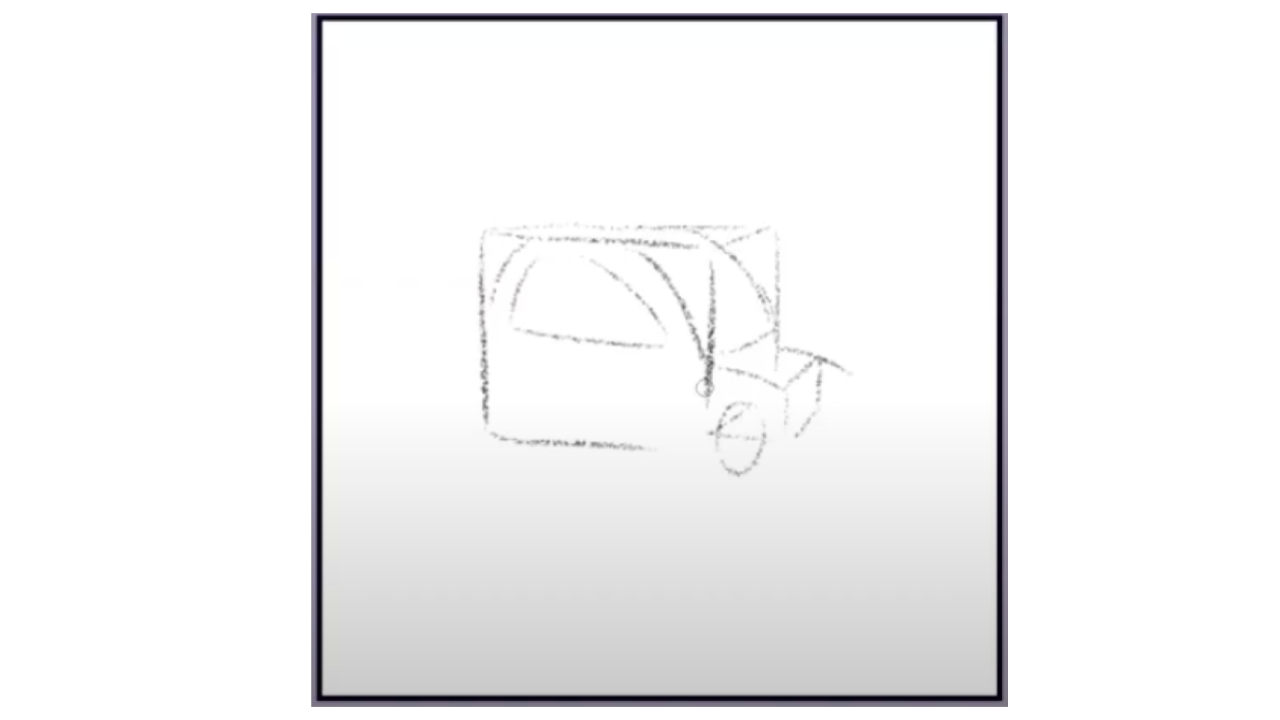
\includegraphics[width=.8\textwidth]{abstraction/figures/expertbox.png}
% \vspace{-0.2in}
%   \caption{An expert demonstrating how box shapes can be used as the basis for drawing nearly any object.}
%   ~\label{fig:expertbox}
%   \vspace{-0.2in}
% \end{figure}

After completing their rough sketch, the experts began adding details. This part of drawing process was much more improvisational; for example, individual members of the group freely colored in areas of the sketch with little or no coordination with other members of the group. In a post-interview, experts noted that the drawing phases did not require as much communication or coordination, since much of the sketch had been previously outlined, reflecting the key concepts of loosely coupled work and maintaining common ground \cite{olson2000distance}.

\subsection{Abstraction Blocks: Making the Abstract Concrete}
From prior work on expert abstraction strategies and our observations of the expert illustrators, we distill these strategies into \textit{abstraction blocks}. We implement these blocks using paper sticky notes as representations of blocking, or chunking, elements that can be shaped, edited, and moved around as desired (Figure \ref{fig:blocks}). We chose to characterize abstraction as abstraction blocks because we expected it would be easy for novices to understand and because it mimics common abstraction strategies used by experts in our chosen domain of drawing \cite{poore1967composition}. While sketches are an abstract representation themselves, novices especially still focus on details rather than exploratory goals during sketching \cite{welch2000sketching}. Encouraging participants to use blocks allows participants to convey rough composition without the need for sketching, emphasizes the spatial relationships between components of a drawing rather than its details, and express a creative vision without worrying about drawing skill or matching the aesthetic style of other collaborators.


\section{Observational Design Study}
\label{sec:abs_study}
In this observational design study, we wanted to observe how groups of people with varying levels of expertise in art would work together on a drawing task, and see how collaboration would be affected by usage of abstraction strategies. While the experts we observed used abstract composition sketches to create the ``undersketch'' of their eventual drawing, we anticipated that most of our participants would not know how to do this. 

\subsection{Method}

\subsubsection{Participants}
Six groups of two to four people ($n=$ 19, 11 female, average age $=$ 28 years) participated in a collaborative drawing task. Participants were recruited from a technology company and local art school through an email advertisement and signed up for scheduled time slots. Though group members were not required to know each other, at least two people from each group had an existing working relationship. The average self-reported drawing experience level was 1.95 ($SD=$ 0.78) out of 4, with 1 being no experience and 4 being expert level. We randomly assigned groups to two conditions: three to \textit{abstraction} and three to \textit{freeform}. Each condition comprised one group of size two, one group of three, and one group of four to explore how communication potentially changes as function of group size. While most groups were co-located, one group in each condition consisted of distributed participants using an online shared canvas (Google Jamboard) and video conferencing (BlueJeans). Observing these distributed groups gave insight on the impact of abstraction on co-located versus remote collaboration. Participants received a \$25 USD gift card for their time. All sessions were video and audio recorded with the experimenter taking note of critical moments during each session.  

\subsubsection{Procedure}
For \textit{abstraction} groups, we first presented a short tutorial of how to use abstraction blocks (Figure \ref{fig:blocks}). Our tutorial explained that participants could use the blocks to represent where a sketch element would be in a drawing. They were free to use text, sketches, or the blocks as they pleased. Groups each made a collective drawing in response to the prompt, ``A scene with a time-traveling tourist.'' We chose a fictional storytelling prompt and drawing task because it does not require any domain knowledge and enables collaborative ideation and interaction \cite{Davis2017}. The task was 20 minutes long and broken into three segments to control for time spent in each part of the process across conditions: five minutes for brainstorming, five minutes for planning and drafting, and ten minutes for drawing. Groups could use paper, pens, pencils, and colored pencils throughout the task. We asked each group to deliver their drawing on one sheet of paper by the end of the study session.

During brainstorming, participants discussed ideas without worrying about drawing yet. Before the planning phase, we gave a short explanation of basic composition concepts and instructed groups to focus on drawing composition during planning. \textit{Abstraction} groups were given standard size and small sticky notes to use and presented with the blocking strategy at this time. Google Jamboard's sticky note feature and pen tools simulated using physical sticky notes and regular analog sketching in the remote sessions. \textit{Freeform} groups were able to plan their drawing in any manner. Following planning, groups collaboratively worked on their drawing for the remainder of the task. Directly after the drawing task, the experimenter replayed recorded critical moments on a computer screen for groups (and through the sharescreen feature for digital groups), asked them to reflect on these clips, and reviewed any additional moments mentioned during the discussion. 

\subsection{Results}
To find emergent themes of how groups interacted with drawing artifacts and each other, we noted interesting behaviors and critical moments in each of the sessions, looking for commonalities across groups and between conditions. We found that groups that used abstraction blocks engaged in more conceptual discussion and worked together in a more flexible manner.

\subsubsection{Abstraction Enabled Integrated Collaboration} 
Compared to freeform sketching, abstraction blocks seemed to help groups form a strong shared understanding of each others' ideas. To represent drawing elements, \textit{abstraction} groups placed sticky notes on their draft paper to create a blueprint of their composition. For example, Group 2 (\textit{abstraction}) put three sticky notes together to represent a focal point (a train) of their drawing while using the smaller sticky notes to represent smaller elements (individual people). These sticky notes were labeled with a brief written description or a small sketch showing what the block was supposed to represent.

\begin{figure*}
\centering
  \vspace{-0.2in}
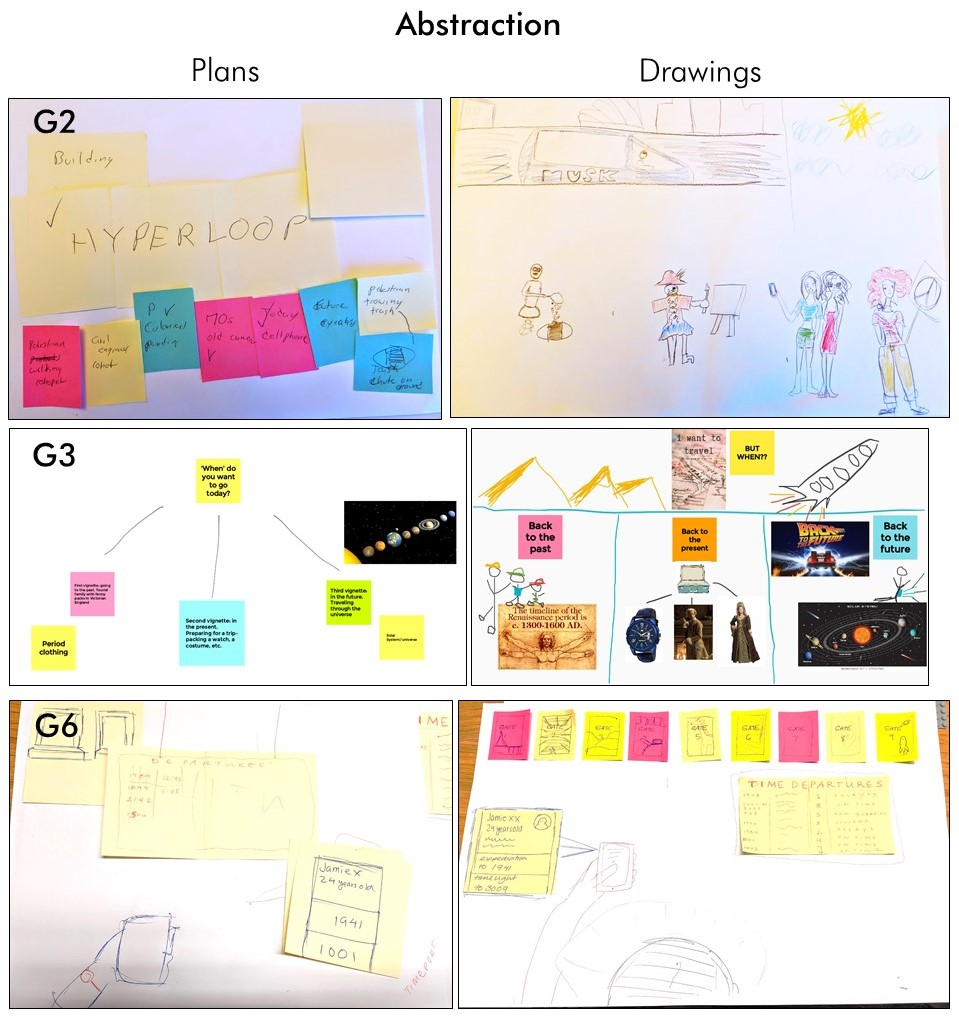
\includegraphics[width=\textwidth]{abstraction/figures/abs.jpg}
% 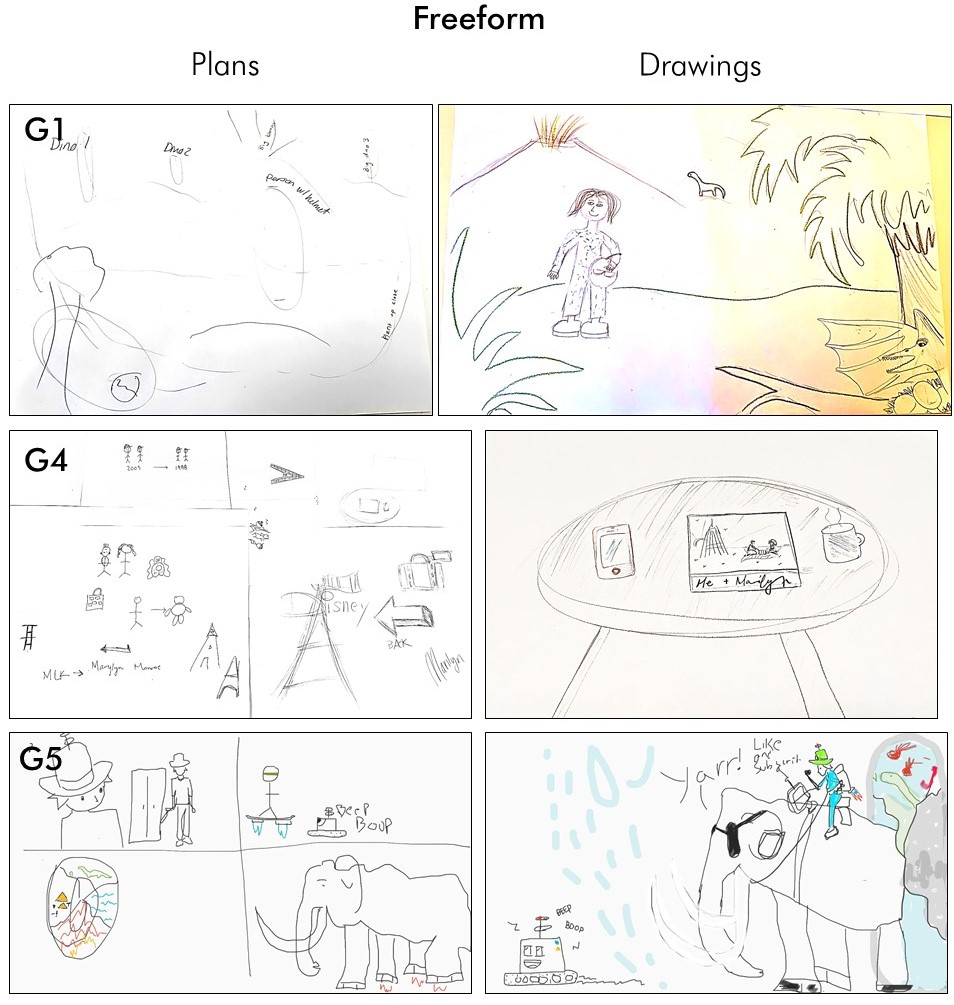
\includegraphics[width=\textwidth]{abstraction/figures/freeform.jpg}
\vspace{-0.3in}
  \caption{\textit{Abstraction} groups developed composition plans from the abstract blocks that formed the basis of their final drawings.}
  ~\label{fig:abs_drawings}
  \vspace{-0.2in}
\end{figure*}

\begin{figure*}
\centering
  \vspace{-0.2in}
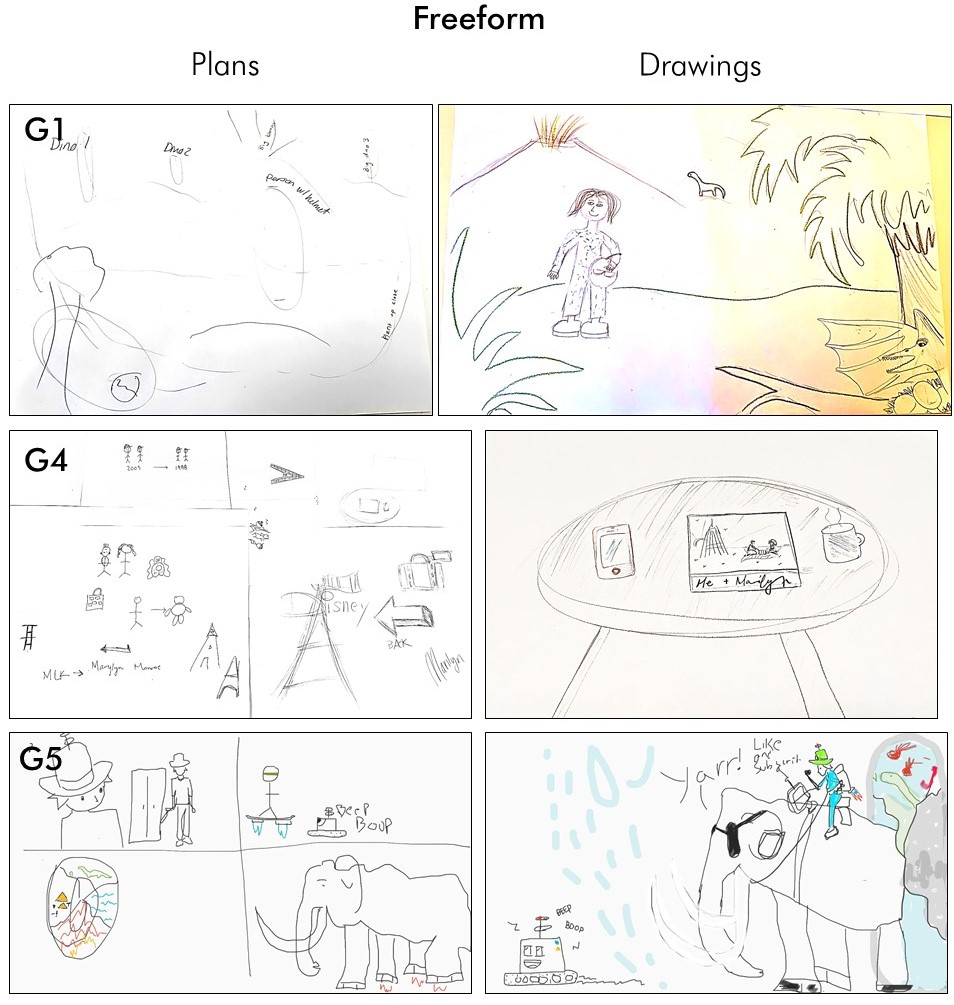
\includegraphics[width=\textwidth]{abstraction/figures/freeform.jpg}
\vspace{-0.3in}
  \caption{\textit{Freeform} groups tended to sketch individual details before deciding on a final composition.}
  ~\label{fig:freeform_drawings}
  \vspace{-0.2in}
\end{figure*}

Similar to the thumbnail sketches created by the experts we observed, abstraction blocks helped anchor discussion by providing shared representations of what members of the group were thinking about: \textit{``I think once someone gave us a visual view of what [they were] thinking, I feel like we all were like ‘Yeah! Perfect'.''} (P5, \textit{abstraction}). P6 (\textit{abstraction}) similarly said in the post-interview that \textit{``everyone has different ways of placing things on paper so once we laid out that this goes here, I think it was helpful for all of us to just visualize the layout of all the things we were talking about.''}

In contrast, Group 1 was the only \textit{freeform} group to make a lightly sketched blueprint of their drawing due to one participant's prior domain knowledge in photography and compositions. 

In other \textit{freeform} groups, participants sketched their own individual drawing elements on separate sheets of paper or divided up their shared drawing sheet into areas ``owned'' by each member of the group (Figure \ref{fig:freeform_drawings}). For example, Group 4 members each sketched their own version of the Eiffel Tower on their scratch paper. 
For \textit{freeform} groups, planning seemed to be oriented around making decisions about specific details of the drawing rather than explore options for the drawing's overall composition.

These differences in how groups approached planning their drawing also affected how they allotted drawing work among individuals. \textit{Abstraction} groups tended to use the blocks they had created as a way to define who should draw what. For example, Group 2 (\textit{abstraction}) assigned each person to draw one of the block elements on their composition plan. They physically checked off the blocks on their plan as they were drawing to mark which ones they completed:

\begin{quote}
    P3: \textit{``I can take `colonial' [people].''}\\ 
    P5: \textit{``We'll take the `today' people on this side.''}\\
    --- Group 2 (\textit{abstraction})
\end{quote}

\textit{Freeform} groups focused instead on smaller, individual elements and focused on the details of these elements. For example, Group 1 (\textit{freeform}) split up their work by individual characters: \textit{``So do you want to start drafting the person and play around with outfits, and I'll do the dinosaurs?''} (P1, \textit{freeform}). However, because \textit{freeform} participants had individually planned portions of the drawing separately from others in their group, they encountered conflicts in their understanding of the drawing's composition as sketching progressed.

One \textit{freeform} participant in Group 5 asked another group member to redraw and switch the orientation of another element during drawing: \textit{``Can you draw the portal on the right because I drew the mammoth from right to left, and this will be very complicated for me to draw it from left to right.''} (P16 \textit{freeform}). There was also sometimes confusion about what each person should work on during drawing. In the post-interview, P13 (\textit{freeform}) said, \textit{``I didn't quite know what I was doing, everyone seem to have their own parts...and I was like 'what should I do?'''}. P14 (\textit{freeform}) also mentioned that he wished his group had done more concrete outlining beforehand so \textit{``people can work more independently instead of having to wait for another part to be done.''} 

\subsubsection{Abstraction Groups Focused on High-Level Decisions}
Groups that used abstract blocks seemed to discuss higher-level concepts like general theme and layouts throughout the drawing process. For example, when talking about how to depict a person looking at a time travel app on his phone, Group 6 (\textit{abstraction}) included light sketches on their blocks (Figure \ref{fig:abs_drawings}) to capture and discuss concepts like point of view, background focus, and scale during planning:

\begin{quote}
    P19: \textit{``Maybe we're still in his point of view, like he's looking at his phone.''}\\
    P17: \textit{``The scale can be small because we probably don't want to get too detailed, but the idea is just to convey that it's a travel app.''}\\
    P18: \textit{``And maybe we can have a thing where it's like zoomed in to show this is what he's holding.''}\\
    --- Group 6 (\textit{abstraction})
\end{quote}

Group 3 (\textit{abstraction}), the digital group, spent their planning time setting high-level goals for their drawing. They made blocks with questions for what they wanted to achieve in their drawing rather than making individual sketches: \textit{``Do you wanna have the main question on the top, and then like three vignettes below?''} (P8, \textit{abstraction})

\begin{figure}[b!]
\centering
  \vspace{-0.25in}
  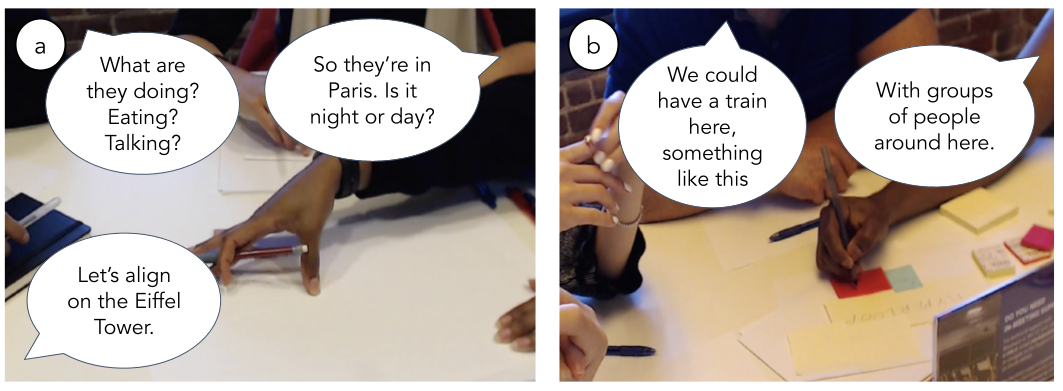
\includegraphics[width=.9\columnwidth]{abstraction/figures/planning.png}
  \caption{(a) \textit{Freeform} groups discussed details early without making concrete sketches until their final drawing. (b) \textit{Abstraction} groups instead used abstract blocks to concretely discuss and sketch a drawing composition.}~\label{fig:tangible}
  \vspace{-0.2in}
\end{figure}

\textit{Freeform} groups instead had a tendency to discuss lower-level details during planning, corroborating findings from prior work \cite{jansson1991design, Little2010, Yu2016}. In Group 5 (\textit{freeform}), participants discussed incremental details for how specific elements should look. For example, when discussing how to show a time traveller coming out of a time travel portal:

\begin{quote}
    P15: \textit{``We could have different futures in the portal, like maybe one where the world is flooded.''}\\
    P14: \textit{``Looks like [P15] has gone in pretty hard on [drawing] the portal...so [P13] should draw the traveler.''}\\
    P15: \textit{``And then [P14] will add lasers to it.''}\\
    P14: \textit{``Yeah like laser accessories.''}\\
    --- Group 5 (\textit{freeform})
\end{quote}

Discussions would often chain together incrementally, adding more details to existing ideas rather than offering new directions to explore. For example, Group 4 (\textit{freeform}) similarly attended to details and discussed the specifics of what their subjects would be doing in their drawing despite being in the planning stage of the study session:

\begin{quote}
    P12: \textit{``What are they doing? Talking?''}\\
    P9: \textit{``Eating?''}\\
    P11: \textit{``Yeah, wine. Eating.''}\\
    P12: \textit{``Coffee?''}\\
    P11: \textit{``No, wine.''}\\
    P9: \textit{``Cheese?''}\\
    P11: \textit{``Yup, cheese. Macarons? Done.''}\\
    --- G4 (\textit{freeform})
\end{quote}

In contrast to the expert group we observed, where improvisational discussion of details occurred during the final stages of drawing, \textit{freeform} groups discussed these details during the early stages of ideation despite being encouraged to plan. For \textit{abstraction} groups, structuring abstraction around blocks oriented discussion around the overall composition of their drawing rather than the specific details of how the drawing should eventually look.

\subsubsection{Abstraction Enabled Flexible Workflows}
Abstraction blocks enabled \textit{abstraction} groups to easily explore alternative layouts and ideas.
\textit{Abstraction} groups described drawings as iterative and malleable, using their planning process to ask new ``what if'' scenarios. For example, while discussing how to draw a train station for time traveling, Group 6 (\textit{abstraction}) moved blocks to reflect their changing concept and even incorporated the blocks in their final drawing so they could continue to iterate and adapt (Figure \ref{fig:abs_drawings}):

\begin{quote}
    P17: \textit{``What if it's like multiple doors to multiple time periods?''}\\
    P19: \textit{``Oh and like this [sticky note] can be like the screen that shows all the departures.''}\\
    P18: \textit{``What if it was like this?''} (Takes a sticky note and moves it to another part of the planning canvas)\\
    --- Group 6 (\textit{abstraction})
    
\end{quote} 

Abstraction blocks were useful for planning, but also for making changes during drawing. For instance, during drawing Group six originally drew a screen in the middle of their page, but because they drew the screen on a block, they moved it further to the right side of the page. When asked their reasoning behind this change, P19 (\textit{abstraction}) said, \textit{``There was a moment [when] we realized that we didn't have enough space so that was a moment where we switched things around''}. Abstraction blocks helped in easily adapting their drawing plan even in the later stages of drawing. 

P17 (\textit{abstraction}) said the blocks felt impermanent: \textit{``When you draw something, it's permanent, but you can move [blocks] around, so you're not really committed.''}. P7 (\textit{abstraction}) also said direct manipulation of blocks helped in getting started: \textit{``Being able to take a sticky note and drag it to where you want it to go, it's so much easier to get started.''} (Figure \ref{fig:tangible}). Some participants thought the abstract blocks resembled other low-fidelity prototyping methods in helping groups view the drawing as piecemeal rather than a fixed whole. In particular, tangible pieces provided structure in building drawing plans: \textit{``It's about being tangible versus intangible so when we see [a block], we grasp onto the idea of that being something''} P18 (\textit{abstraction}). The flexibility in creating malleable chunks framed the drawing as impermanent, helping groups easily explore different ideas and concepts even during the final drawing phase. 

P7 (\textit{abstraction}) also said the abstraction blocks helped in getting started on the drawing: \textit{``it helped in [overcoming] that sort of blank page...and you're so daunted that you don't know how to get started...Then when you have a plan you can just get going on the drawing. There wasn't much discussion about what to do in the final stage because it had already been planned out.''} (P7, \textit{abstraction}).

In contrast, \textit{freeform} groups worked linearly and were often more hesitant to commit to and revise ideas. 
Sketching, even at a draft stage, was viewed as representing a permanent decision. In the post-interview, P12 (\textit{freeform}) mentioned expressing many ideas verbally, but being hesitant to start their drawing: \textit{``Nothing was concrete on the paper. So it was like we're just spitballing, but once you actually put ink to paper then it's like oh now we need to actually do it.''} Group 4 (\textit{freeform}) iterated on specific drawing elements individually (Figure \ref{fig:freeform_drawings}) because sketches on a shared sheet felt more permanent and committal. They aimed to form verbal consensus rather than exploring ideas the way \textit{abstract} groups did (Figure \ref{fig:tangible}). Here they discuss drawing a picture showing the time traveller posing with a historical figure:

\begin{quote}
    P9: \textit{``Do we want to fill the whole page or do we want to do a frame?''}\\
    P11: \textit{``Ooh let's frame it.''}\\
    P9: \textit{``So we agreed on a picture, yes?''}\\
    P10: \textit{``A picture within a picture? So is this like a postcard?''}\\
    P9: \textit{``So someone is like holding the postcard-''}\\
    P12: \textit{``Hands. Yes. I like that.''}\\
    --- Group 4 (\textit{freeform})
\end{quote}

Despite the fact that sketching is often useful as an abstraction tool \cite{Buxton2007,Tversky2009}, \textit{freeform} participants in our study still viewed sketching as costly and permanent, akin to final drawing. By providing \textit{abstraction} participants with a way to move their work around, abstract blocks instead made sketching together a more flexible and less daunting process.


\section{Discussion \& Future Work}
We investigated how directly manipulable abstract blocks affect communication in collaborative sketching. In an observational design study, we found that abstract blocks gave groups a way to break down drawing compositions through movable, simple shapes that de-emphasized details and permanence. They allowed \textit{abstraction} groups to communicate higher-level concepts and explore different ideas and compositions relative to \textit{freeform} groups, which used planning phases to discuss more superficial details rather than compositional concepts. In this section, we discuss the implications of these findings for future creativity support tools.

\subsection{Tools for Supporting Abstract Blocking}
This chapter investigated how scaffolding abstraction through abstract blocks affects exploration and communication in the task of collaborative drawing. 
In any collaborative task, communication can leave ephemeral, intangible artifacts that aid groups in coordinating actions and developing rapport \cite{Davis2017,Davis2016}. For example, group dynamic and physical gestures are important for ideation and building consensus in collaborative drawing tasks \cite{Bly1988, Tang1991}. In our observations, groups used both verbal and non-verbal forms of communication (like gesturing) to make decisions and share ideas \cite{goldin1999}. However, for \textit{abstraction} groups, abstract blocks helped participants concretely express intangible ideas through the placement of directly manipulable shapes, giving groups a malleable visualization of a concept that groups could modify as they conversed. The tangibility of making abstract concepts feel more concrete and importantly, changeable, seemed to be the primary benefit of abstraction blocks.

Groups could, of course, use blocking and similar abstraction strategies without a need for physical blocking tools. However, we observed in our study that \textit{freeform} groups did not use such strategies with the exception of one group who had prior experience in composition concepts through photography. Though sketches are meant to be blocking tools themselves, novices especially do not often separate exploratory sketching from refined drawing \cite{welch2000sketching}, as we observed in \textit{freeform} groups. When a concrete abstraction tool---abstract blocks---was made available, \textit{abstraction} groups were more inclined to create abstract representations. Some groups chose to use text to label blocks, others chose to lightly sketch, but importantly, \textit{abstraction} groups did not decorate blocks with heavy detail. Abstract blocks may have helped form common understanding of the drawing among collaborators \cite{olson2000distance}, helping groups maintain discourse on higher-level concepts.

Abstraction through abstract blocks may be even more beneficial in online settings where intangible communication is difficult. In such settings, groups must rely on technological affordances to effectively collaborate \cite{Hollan1992,Jensen2018}. 
Future collaborative tools could explicitly encourage abstract blocking, as opposed to requiring creators to figure out how to create abstract representations of their work themselves through existing tools (\textit{e.g.}, shape tools in Microsoft PowerPoint or Adobe Photoshop). 
One might also imagine creativity support tools where abstraction-oriented tools and detail-oriented tools can be used in a complementary manner. Our study also showed that there is a time and place for both kinds of representations in a collaborative creative task, and that there is value in being able to move between abstract and concrete representations of a drawing. Rather than needing two separate creativity tools---one for drafting a prototype and one for generating a final creative work---future work might investigate how a tool could help a group seamlessly navigate between two views of the same work.

\subsection{Supporting Creative Collaboration}
Our studies were done at a relatively small scale; abstract blocks could also support structured, large-scale crowdsourcing workflows. One way people seek to collaborate with a crowd in creative work is through asking for feedback or guidance online through discussion forums or creative communities \cite{kuznetsov2010rise,settles2013,wasko2005should} like Behance (www.behance.com). Much of the exchange and communication occurs via text comment feedback and relies on the creator to interpret suggestions, make changes, and update their work. Methods for structuring communication and exchange among crowd collaborators include assessment \cite{Dow2012} and framing \cite{hicks2016framing} prompts, but much of creative work relies on being to \textit{see} and understand changes. In our observations, we saw that collaborators formed a consensus around sketch ideas through abstract blocking. Similar to bringing in examples as a way to show ``something like this'' \cite{kang2018paragon}, abstract blocks enable quick ways to visually demonstrate ideas without focusing on details.

We also observed that groups used abstract blocks as a way to delegate tasks among collaborators, using the blocks as structured components for each collaborator. At a larger scale, abstract blocking could aid in managing input from a large number of contributors. For example, in leader-facilitated crowdsourcing approaches such as flash teams, a leader could assign modular tasks to a team through blocks \cite{Retelny2014,Salehi2018,Valentine2017} or signal which parts of a creative work are open for collaboration \cite{kim2014ensemble}. In remixing communities, contributors might use blocking to build upon certain structural components of an existing project \cite{Resnick2009}. From a social perspective, abstract blocks can also give a tangible way for interactively exploring ideas, which could be particularly useful in creative livestreams where a crowd can engage with an artist and contribute ideas beyond text chat suggestions and audience voting games \cite{Fraser2019}. Future work should examine how abstract blocking might impact communication at a larger-scale across domains.

\subsection{Rich Abstraction or Simple Details?}
One limitation of using abstract blocks was a decrease in improvisation. Serendipitous creativity can occur through collaborators building and improvising off others' ideas \cite{Davis2017,Davis2016}. We saw this in the \textit{freeform} groups where groups would chain ideas together, adding on different details as the group discussed. Because \textit{abstraction} groups created a concrete composition plan ahead of drawing, we observed more expedient drawing, but with less improvisation overall. However, we did observe improvisation and exploration during the planning process when groups were first discussing sketch ideas. \textit{Abstraction} groups explored alternative composition ideas rather than details early on, reflecting the expert process we observed. One area for future work is examining what level of abstraction is appropriate at different stages of creative work. Could abstraction blocks be used to also specify concrete details? This could allow both for exploration of high-level compositions as well as exploration of lower-level details while removing the need for higher-fidelity sketching. Tools could provide different modes for different levels of abstraction, similar to multi-layered interfaces that adaptively disclose functionality as the user progresses \cite{shneiderman2002promoting}.

Another limitation to using abstract blocks is it is unclear \textit{how much} detail should be abstracted. Some groups in our study simply used text labels on blocks to communicate an idea. Others used lightly sketched images. One group used image search to provide a reference for their idea. Each of these representations might differentially impact communication and understanding of the ideas presented. In addition, most \textit{abstraction} groups did not discuss nuanced composition details such as the direction a character is facing or their position in the drawing. Instead, much of the discussion emphasized placement since the abstract blocks focused on adjusting the sketch's overall layout. We saw more of a discussion of these details in the \textit{freeform} group. 

Our observational design study presents several opportunities for how tools might implement abstraction strategies such as abstract blocking. The first is in supporting large-scale collaboration. We observed how tangible and malleable blocks helped groups communicate and iterate upon abstract, exploratory ideas. One question for future research is how abstract blocks might support communicating composition details while maintaining flexibility and high-level focus without compromising the benefits afforded by removing detail in the first place. Another opportunity is in comparing the use of abstraction blocks in individuals versus a group and seeing how exploration strategies might change based on the level of communication and collaboration. Lastly, we examined abstraction blocks in sketching, but the concept could apply to any domain where high-level goals can be broken into chunks. Future work should examine the nature of abstraction and how abstraction blocks might be utilized in domains outside of visual work.

\subsubsection{Summary}
In this chapter, we describe and evaluate using abstraction blocks, a technique where visual content is \emph{abstracted} to simple shapes to facilitate communication and collaboration on visual creative work such as drawings. By abstracting elements of visual work, we found in an observational design study that people are more likely to explore high-level concepts such as composition and perspective and are less likely to fixate on details of an early idea. Collaborative tasks rely on effective communication between contributors. For novices especially, communicating higher-level goals and changes can be challenging without domain or procedural knowledge. Abstraction blocks scaffold this communication, using simple shapes as a flexible medium to create conceptual chunks rather than detailed sketches. This abstraction makes the invisible visible and the intangible tangible. Collaborative creativity support systems, both for visual creative work and beyond, should include mechanisms for attuning users to the right level of abstraction to explore and communicate higher-level concepts.

\subsubsection{Acknowledgements}
We thank our research participants for their time and efforts. This research was funded in part by Adobe Research.

This chapter, in part, is being prepared for submission for publication by Tricia J. Ngoon, Joy O. Kim, and Scott Klemmer. The dissertation author was the primary investigator and author of this material.